\documentclass[11pt]{article}
\usepackage[a4paper,landscape,margin=0.72in]{geometry}
\usepackage[T1]{fontenc}
\usepackage{lmodern,amsmath,amssymb,graphicx,hyperref}
\title{Separable quintic: affine and projective point domains}
\author{Formal proof packet}
\date{28 October 2026}
\begin{document}
\maketitle
\noindent This packet records a checked theorem with a visible separability hypothesis. It contains no experiment, target result, or cost ratio. The Lean source, compiler log, editable SVG, and CSV gate table accompany this PDF.

\section*{Checked statement and argument}
Let $K$ be any field and $f(X)=X^5+a_3X^3+a_2X^2+a_1X+a_0$. If $f$ is separable, the pinned Lean proof extracts $t,u\in K[X]$ with $f=tu$, $t$ prime, and $t\nmid u$. The quintic has degree five and is not a unit, so it has an irreducible factor. Separability supplies squarefreeness and excludes that factor from the cofactor. The existing checked Eisenstein lemma then makes $Y^2-f(X)$ irreducible over $K[X][Y]$.

The new theorems establish that $K[X,Y]/(Y^2-f(X))$ is a domain, its localization at any rational point satisfying $y^2=f(a)$ is a domain, and the corresponding actual weighted-$\operatorname{Proj}$ point stalk is a domain. The one-variable equivalence \texttt{MvPolynomial.uniqueAlgEquiv} identifies the extracted factor with the actual quintic representation. No characteristic assumption is needed for this domain statement. The earlier local norm-order theorem still requires its stated hypotheses, including an actual DVR.

\section*{Verification boundary}
Direct compilation used pinned Lean 4.34.1 and Mathlib revision
\par\noindent\texttt{d13f23b723b8a846827a245b89c10fc7d3f11612}.
The command \texttt{TMPDIR=/dev/shm lake env lean Common22SeparableAffineDomain.lean} exited zero. All seven printed axiom audits list only \texttt{propext}, \texttt{Classical.choice}, and \texttt{Quot.sound}; no \texttt{sorryAx}. Two nonfatal style-linter messages recommend \texttt{let} in place of \texttt{letI}. Lean source SHA-256:
\par\noindent{\small\texttt{897099465cefd0afcf7a55668267fb56a46b91b7356a5594f17de6a6a680b602}}.

The exact next local geometry gate is principality of the evaluation maximal ideal in the nonbranch stalk; the checked domain alone does not establish a DVR or order formula. Formula-specific norm transport, global principal-divisor/$\mathrm{Pic}^0$ transport, and compiled Rust semantics are open. An odd-degree proof without separability is also open in this formal line. The CSV preserves these statuses for independent review.

\clearpage
\section*{Proof dependencies and open gates}
\begin{center}
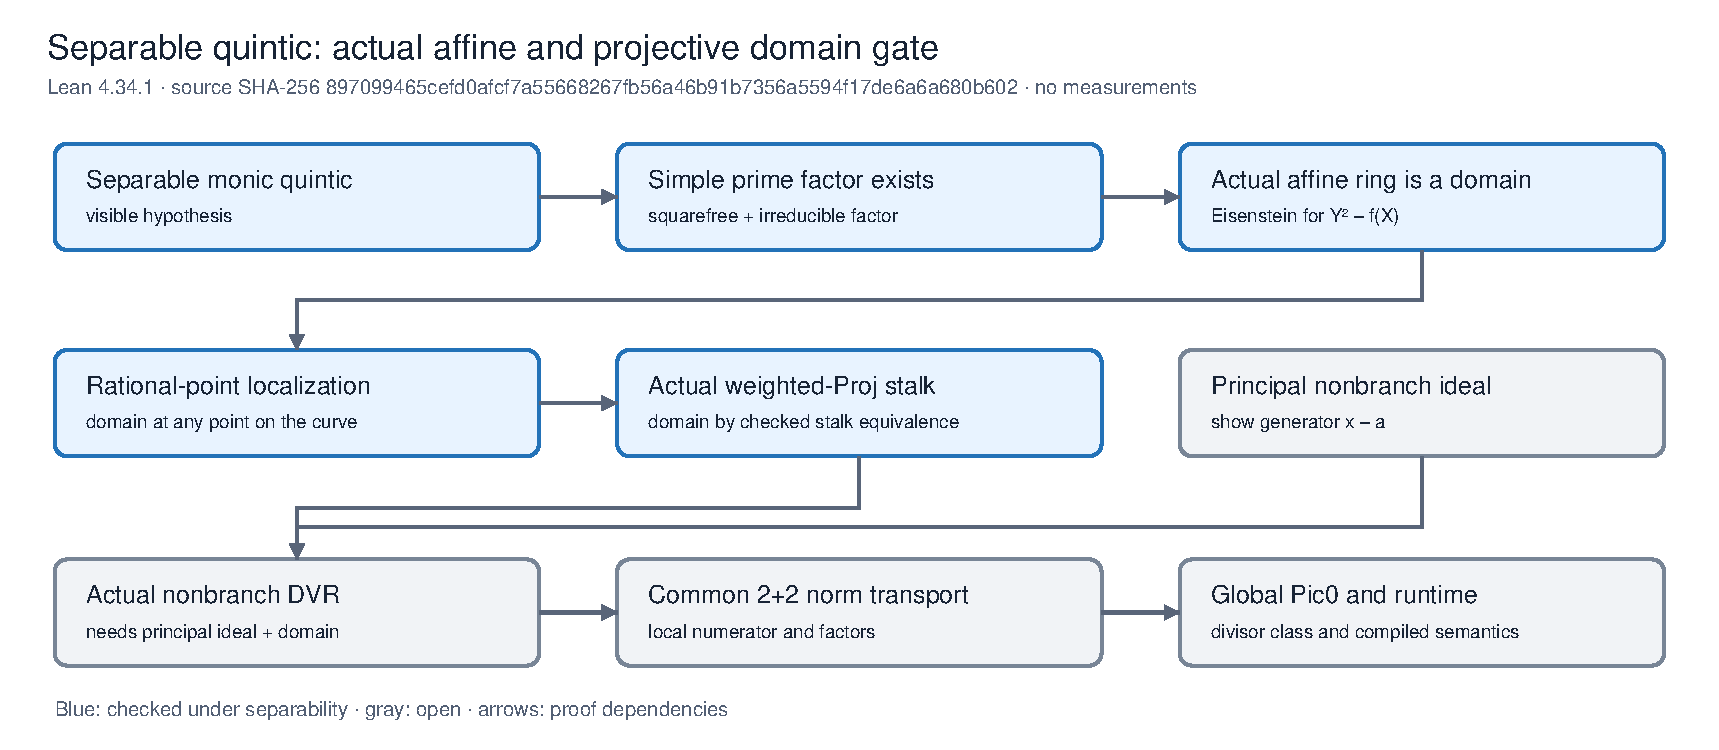
\includegraphics[width=0.96\textwidth,height=0.76\textheight,keepaspectratio]{separable-affine-domain-figure.pdf}
\end{center}
\noindent Blue nodes are checked under separability. Gray nodes are open. Arrows show proof dependencies, not measured performance.
\end{document}
